\documentclass[11pt]{article}

\usepackage{acl}
\usepackage{pdfpages}
\usepackage{hyperref}
\usepackage{fancyvrb}

% Standard package includes
\usepackage{times}
\usepackage{latexsym}

% For proper rendering and hyphenation of words containing Latin characters (including in bib files)
\usepackage[T1]{fontenc}
\usepackage[ngerman]{babel}

% This assumes your files are encoded as UTF8
\usepackage[utf8]{inputenc}

% This is not strictly necessary, and may be commented out,
% but it will improve the layout of the manuscript,
% and will typically save some space.
\usepackage{microtype}

\title{Unicorn: Reasoning about Configurable System Performance through the Lens of Causality \\[16px] \normalfont{Reproduktion und Evaluation}}

\author{
  Alexander Vödisch \\
  \texttt{av21vupu@studserv.uni-leipzig.de} \\
}

\begin{document}

\maketitle

\begin{abstract}
In dieser Ausarbeitung werden die Ergebnisse von [ref] repliziert und evaluiert.
\end{abstract}

\section{Einführung}

Moderne Computersysteme sind oft aus einer Vielzahl von konfigurierbaren Komponenten aufgebaut, deren Zusammensetzung kritisch für die Systemperformance ist.\footnote{Unter (System-)Performance werden alle Leistungsmerkmale eines Systems wie beispielsweise Durchsatz und Energieverbrauch zusammengefasst.} Da die optimale Konfiguration dieser Komponenten hardwareabhängig sein kann und insbesondere in Kombination zu Pipelines der Konfigurationsraum exponentiell wachsen kann, sind spezielle Algorithmen notwendig, um Nutzer solcher Systeme bei der Definition möglichst optimaler Konfigurationen zu unterstützen.

Das Ziel von \textsc{Unicorn} ist es, für konfigurierbare Systeme die optimalen Konfigurationen bezüglich eines vom Nutzer definierten Merkmals (z.\,B. Leistung, Energieverbrauch, Inferenzzeit) zu finden und im Zuge dessen einen kausalen Graphen zu generieren, der als Modell auch auf bisher unbekannte Harware übertragen werden kann.

Im Gegensatz zu Modellen, die beispielsweise auf Regression basieren und lediglich den Einfluss individueller Konfigurationsoptionen messen, bietet \textsc{Unicorn} den Vorteil, dass nicht die Korrelation von Konfigurationsoptionen zur Vorhersage von guten Konfigurationen, sondern die kausalen Zusammenhänge der einzelnen Optionen für die Entwicklung des Modells genutzt werden. Dadurch kann das Modell auch in unbekannten Environments genutzt werden, wo korrelationsbasierte Performance-Influence-Modelle oft nur unzuverlässige Vorhersagen treffen.

\section{Funktionsweise}

\begin{figure}[tp!]
  \centering
  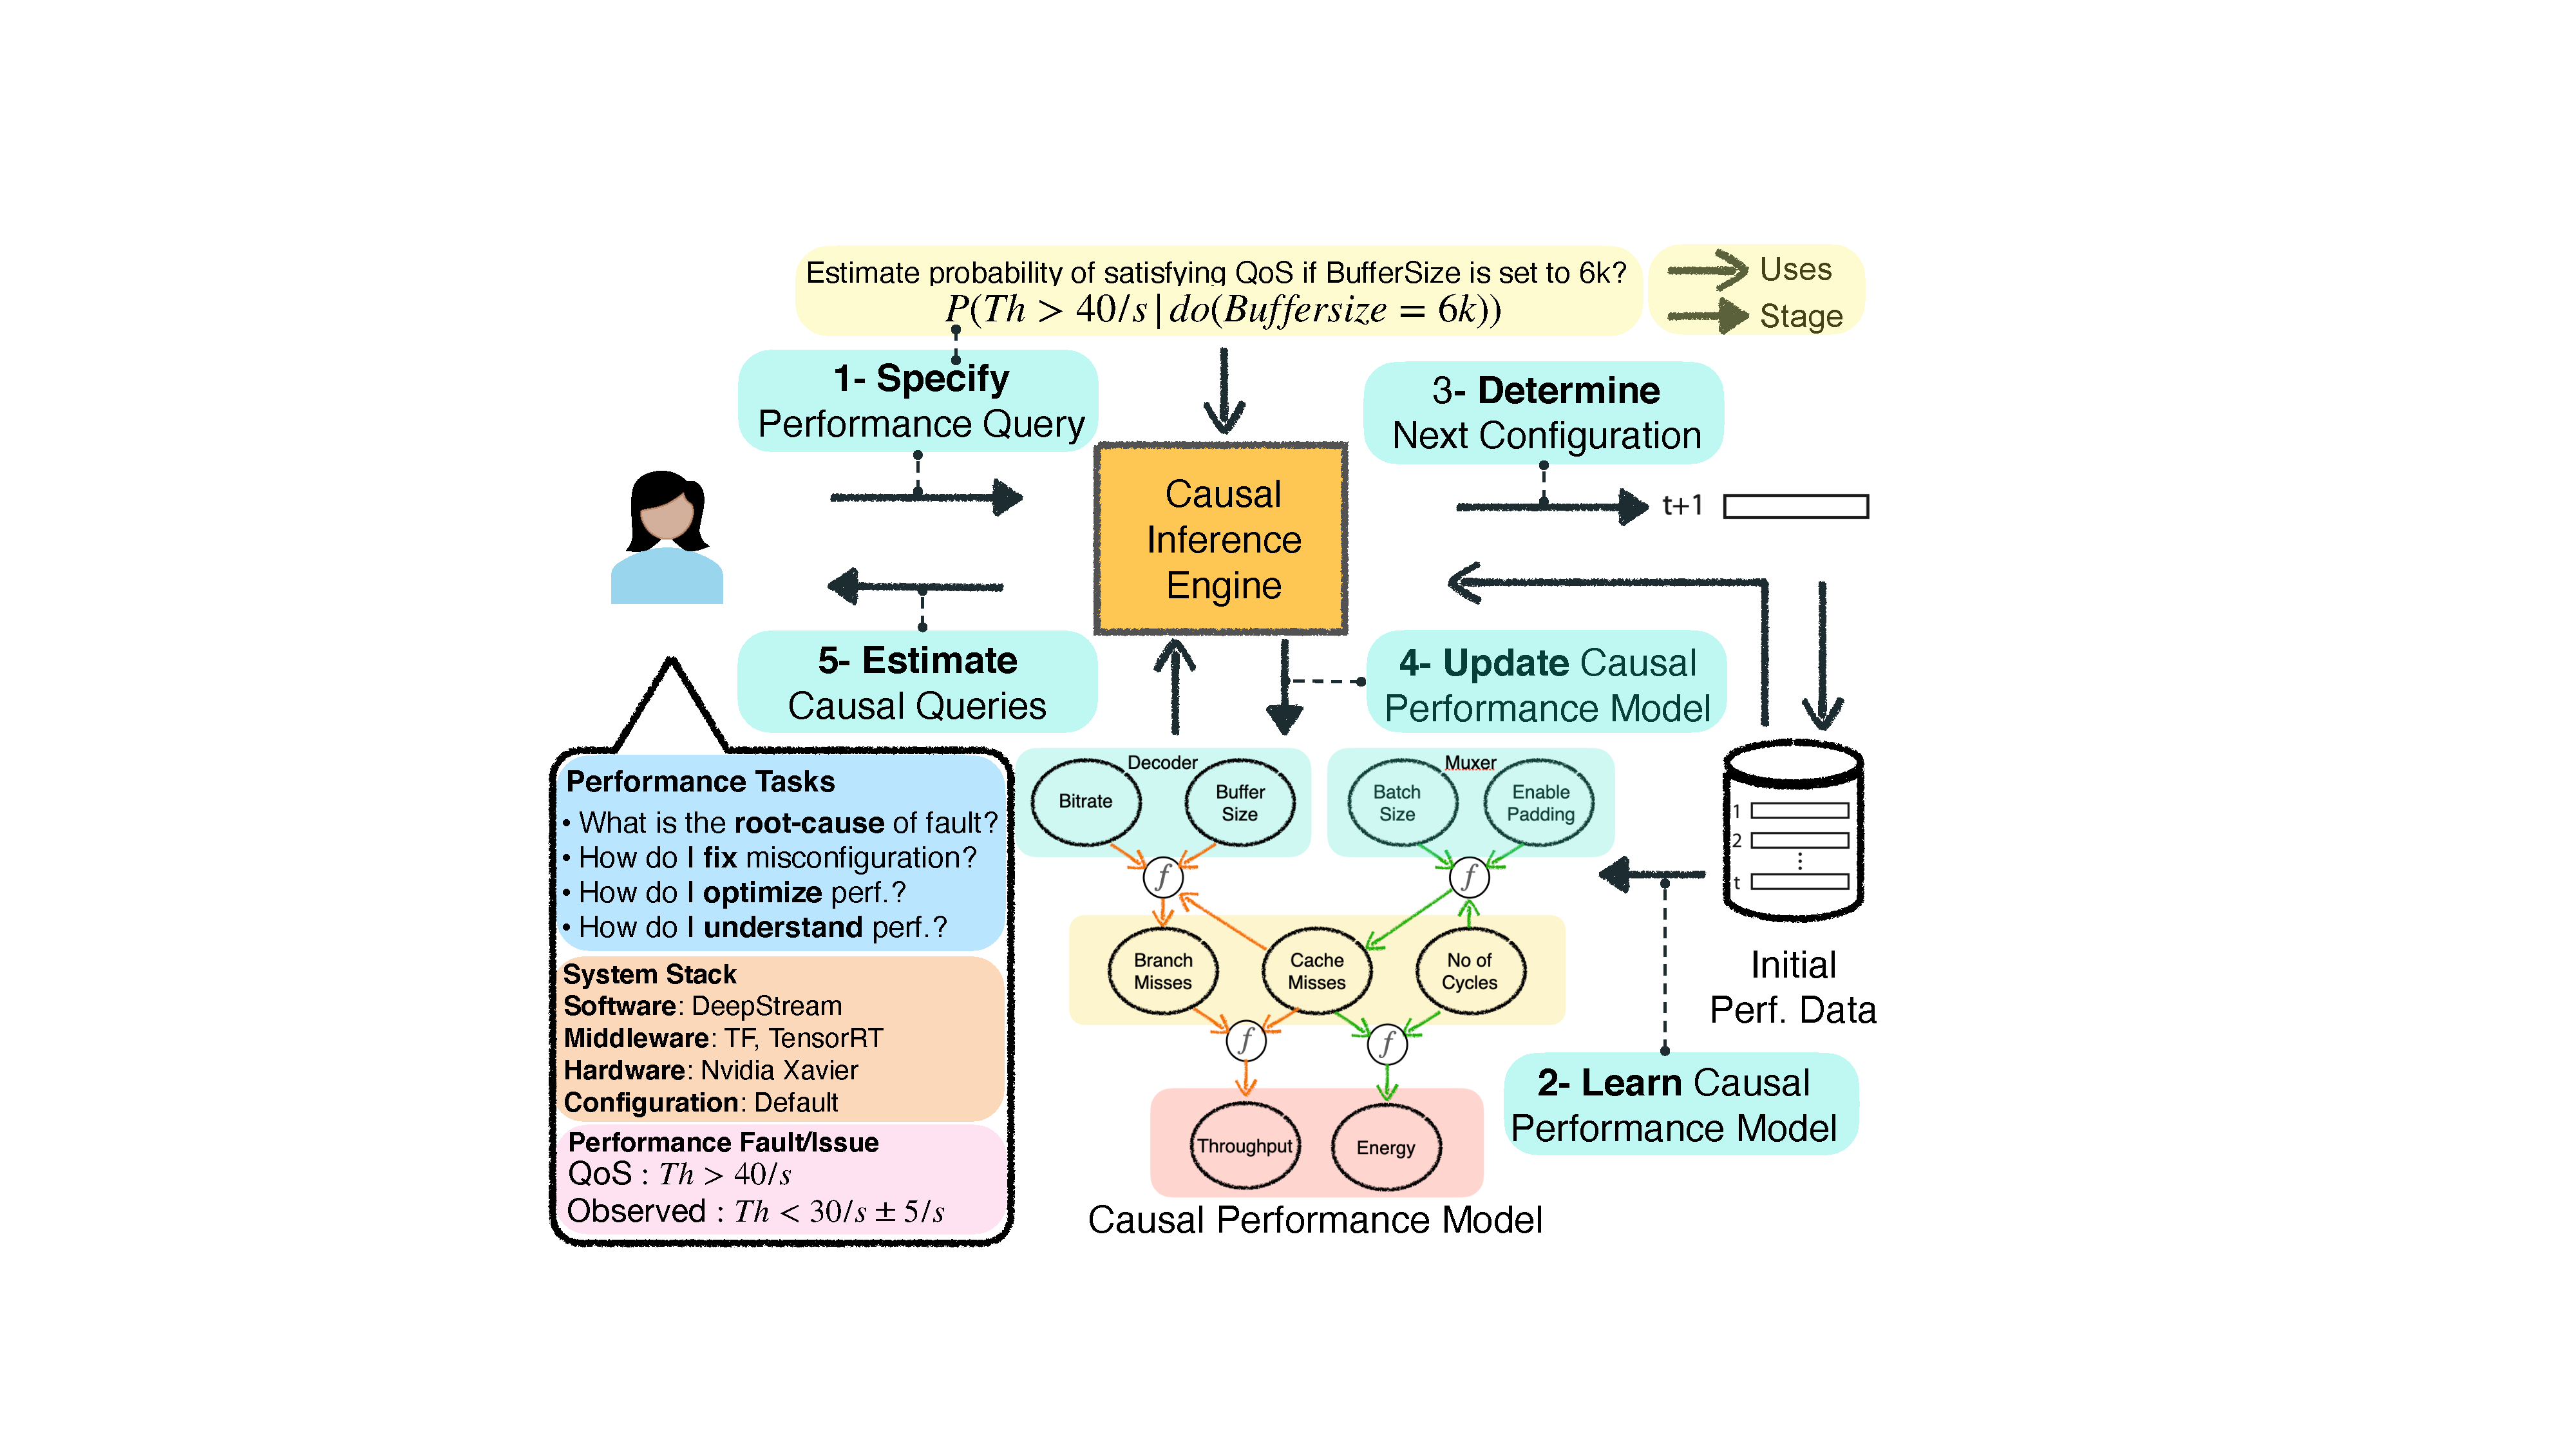
\includegraphics[width=\linewidth]{./img/UnicornOverview.pdf}
  \caption{\small {}}

  \label{}
\end{figure}

\textsc{Unicorn} ermöglicht sowohl das Debuggen als auch auch das Optimieren von Systemkonfigurationen. Hierzu definieren die Autoren ein kausales Modell das auf probabilistischen graphischen Modellen basiert. Diese kausalen Graphen bestehen aus

\begin{itemize}
  \itemsep0em
  \item Performance-Variablen als Knoten für mögliche Konfigurationsparameter (z.\,B. \texttt{Birate}, \texttt{Buffer Size} oder \texttt{Batch Size}),
  \item funktionalen Knoten, die funktionale Abhängigkeiten zwischen den Performance-Variablen modellieren,
  \item kausalen Verbindungen zwischen den Performance-Variablen und den funktionalen Knoten und
  \item Nebenbedingungen, um notwendige Einschränkungen bei der Modellbildung zu definieren (z.\,B. dürfen \texttt{Cache Misses} nur positive ganzzahlige Werte annehmen).
\end{itemize}

\begin{figure}[tp!]
  \centering
  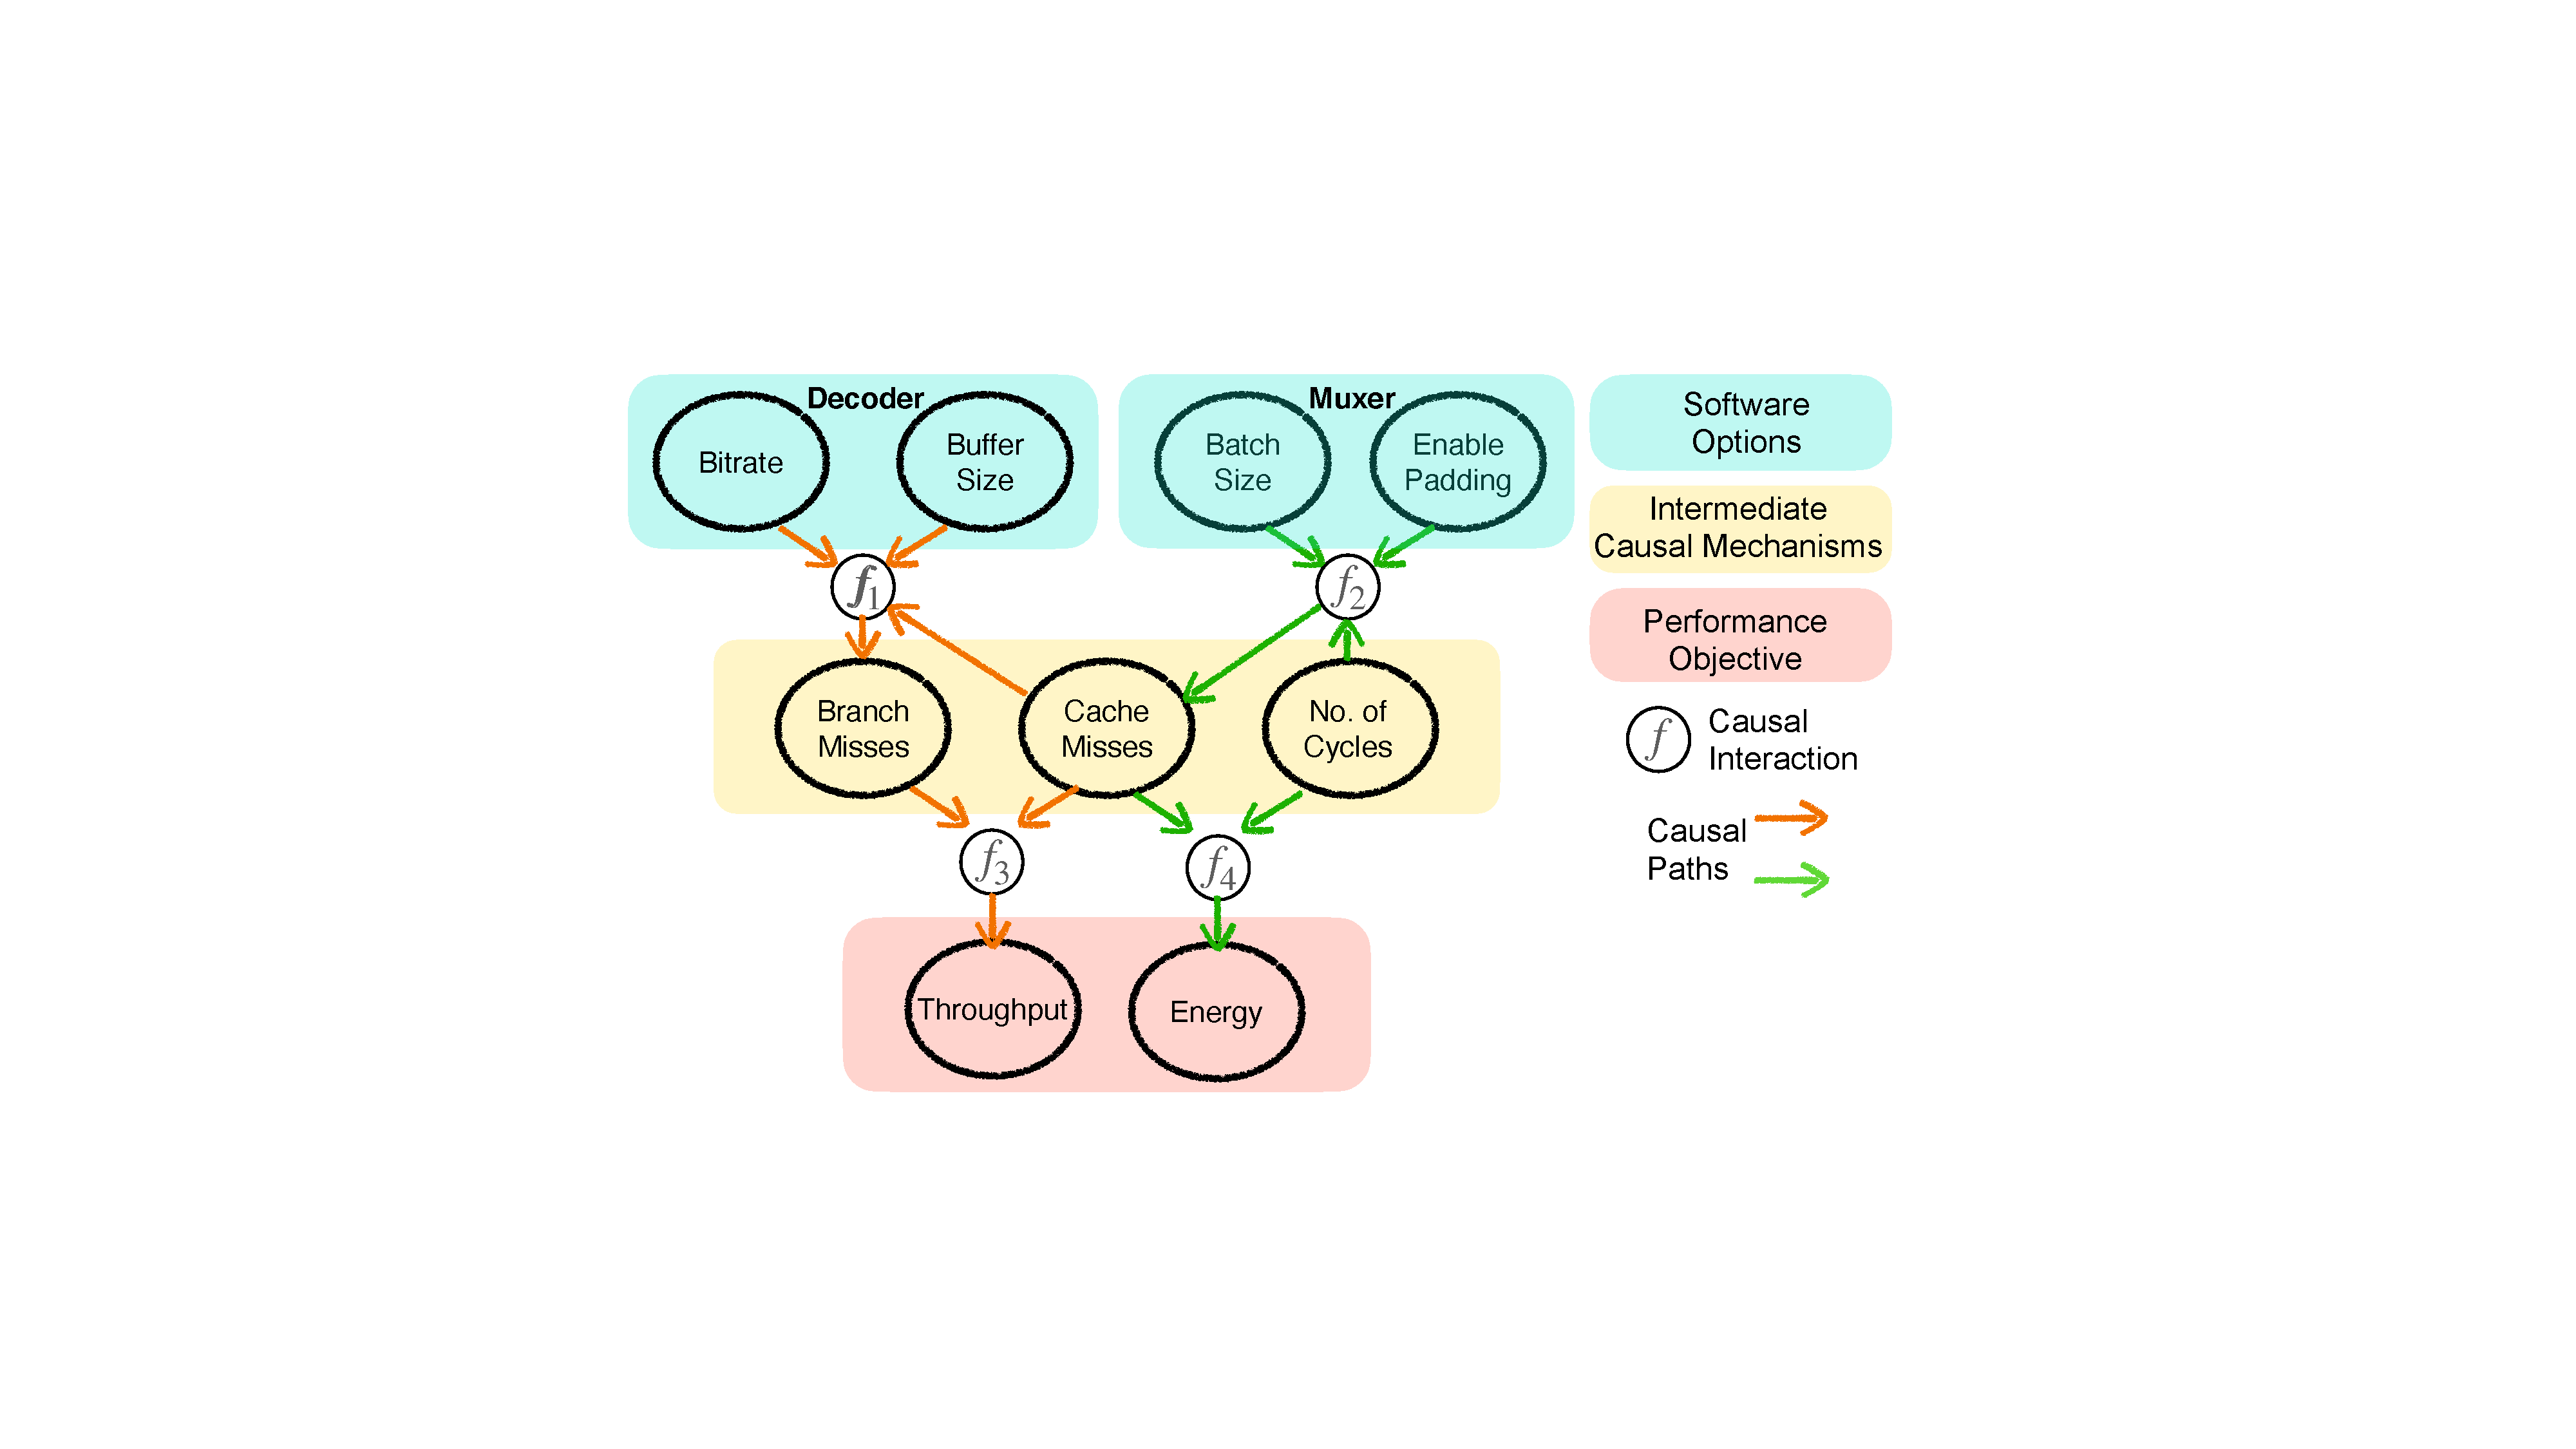
\includegraphics[width=\linewidth]{./img/CausalModelExample.pdf}
  \caption{\small {}}

  \label{}
\end{figure}

\textsc{Unicorn} arbeitet in 5 Schritten:
\begin{enumerate}
  \itemsep0em
  \item Spezifikation der Optimierungsanforderung als Klartext durch den Nutzer
  \item Lernen des kausalen Modells mittels vordefinierter Anzahl an Musterkonfigurationen: Hierfür wird der \textit{Fast Causal Inference}-Algorithmus [ref] genutzt, um Kanten von dem zunächst vollständigem probabilistischen Graphen entsprechend der Nebenbedingungen zu entfernen und ungerichtete Kanten entsprechend der kausalen Einflüsse der Performance-Variablen auszurichten.
  \item Bestimmung der Folgekonfiguration und Messen der Systemperformance: Für die Folgekonfiguration werden diejenigen Performance-Variablen angepasst, die kausal am stärksten Zusammenhängen, um den Lernprozess zu beschleunigen (\textit{Active Learning}).
  \item Inkrementelles Update des kausalen Modells
  \item Wiederholung der Schritte 3 und 4 bis ein vordefiniertes Limit (z.\,B. Laufzeit) überschritten wurde und anschließend Ausgabe
\end{enumerate}

\begin{figure}[tp!]
  \centering
  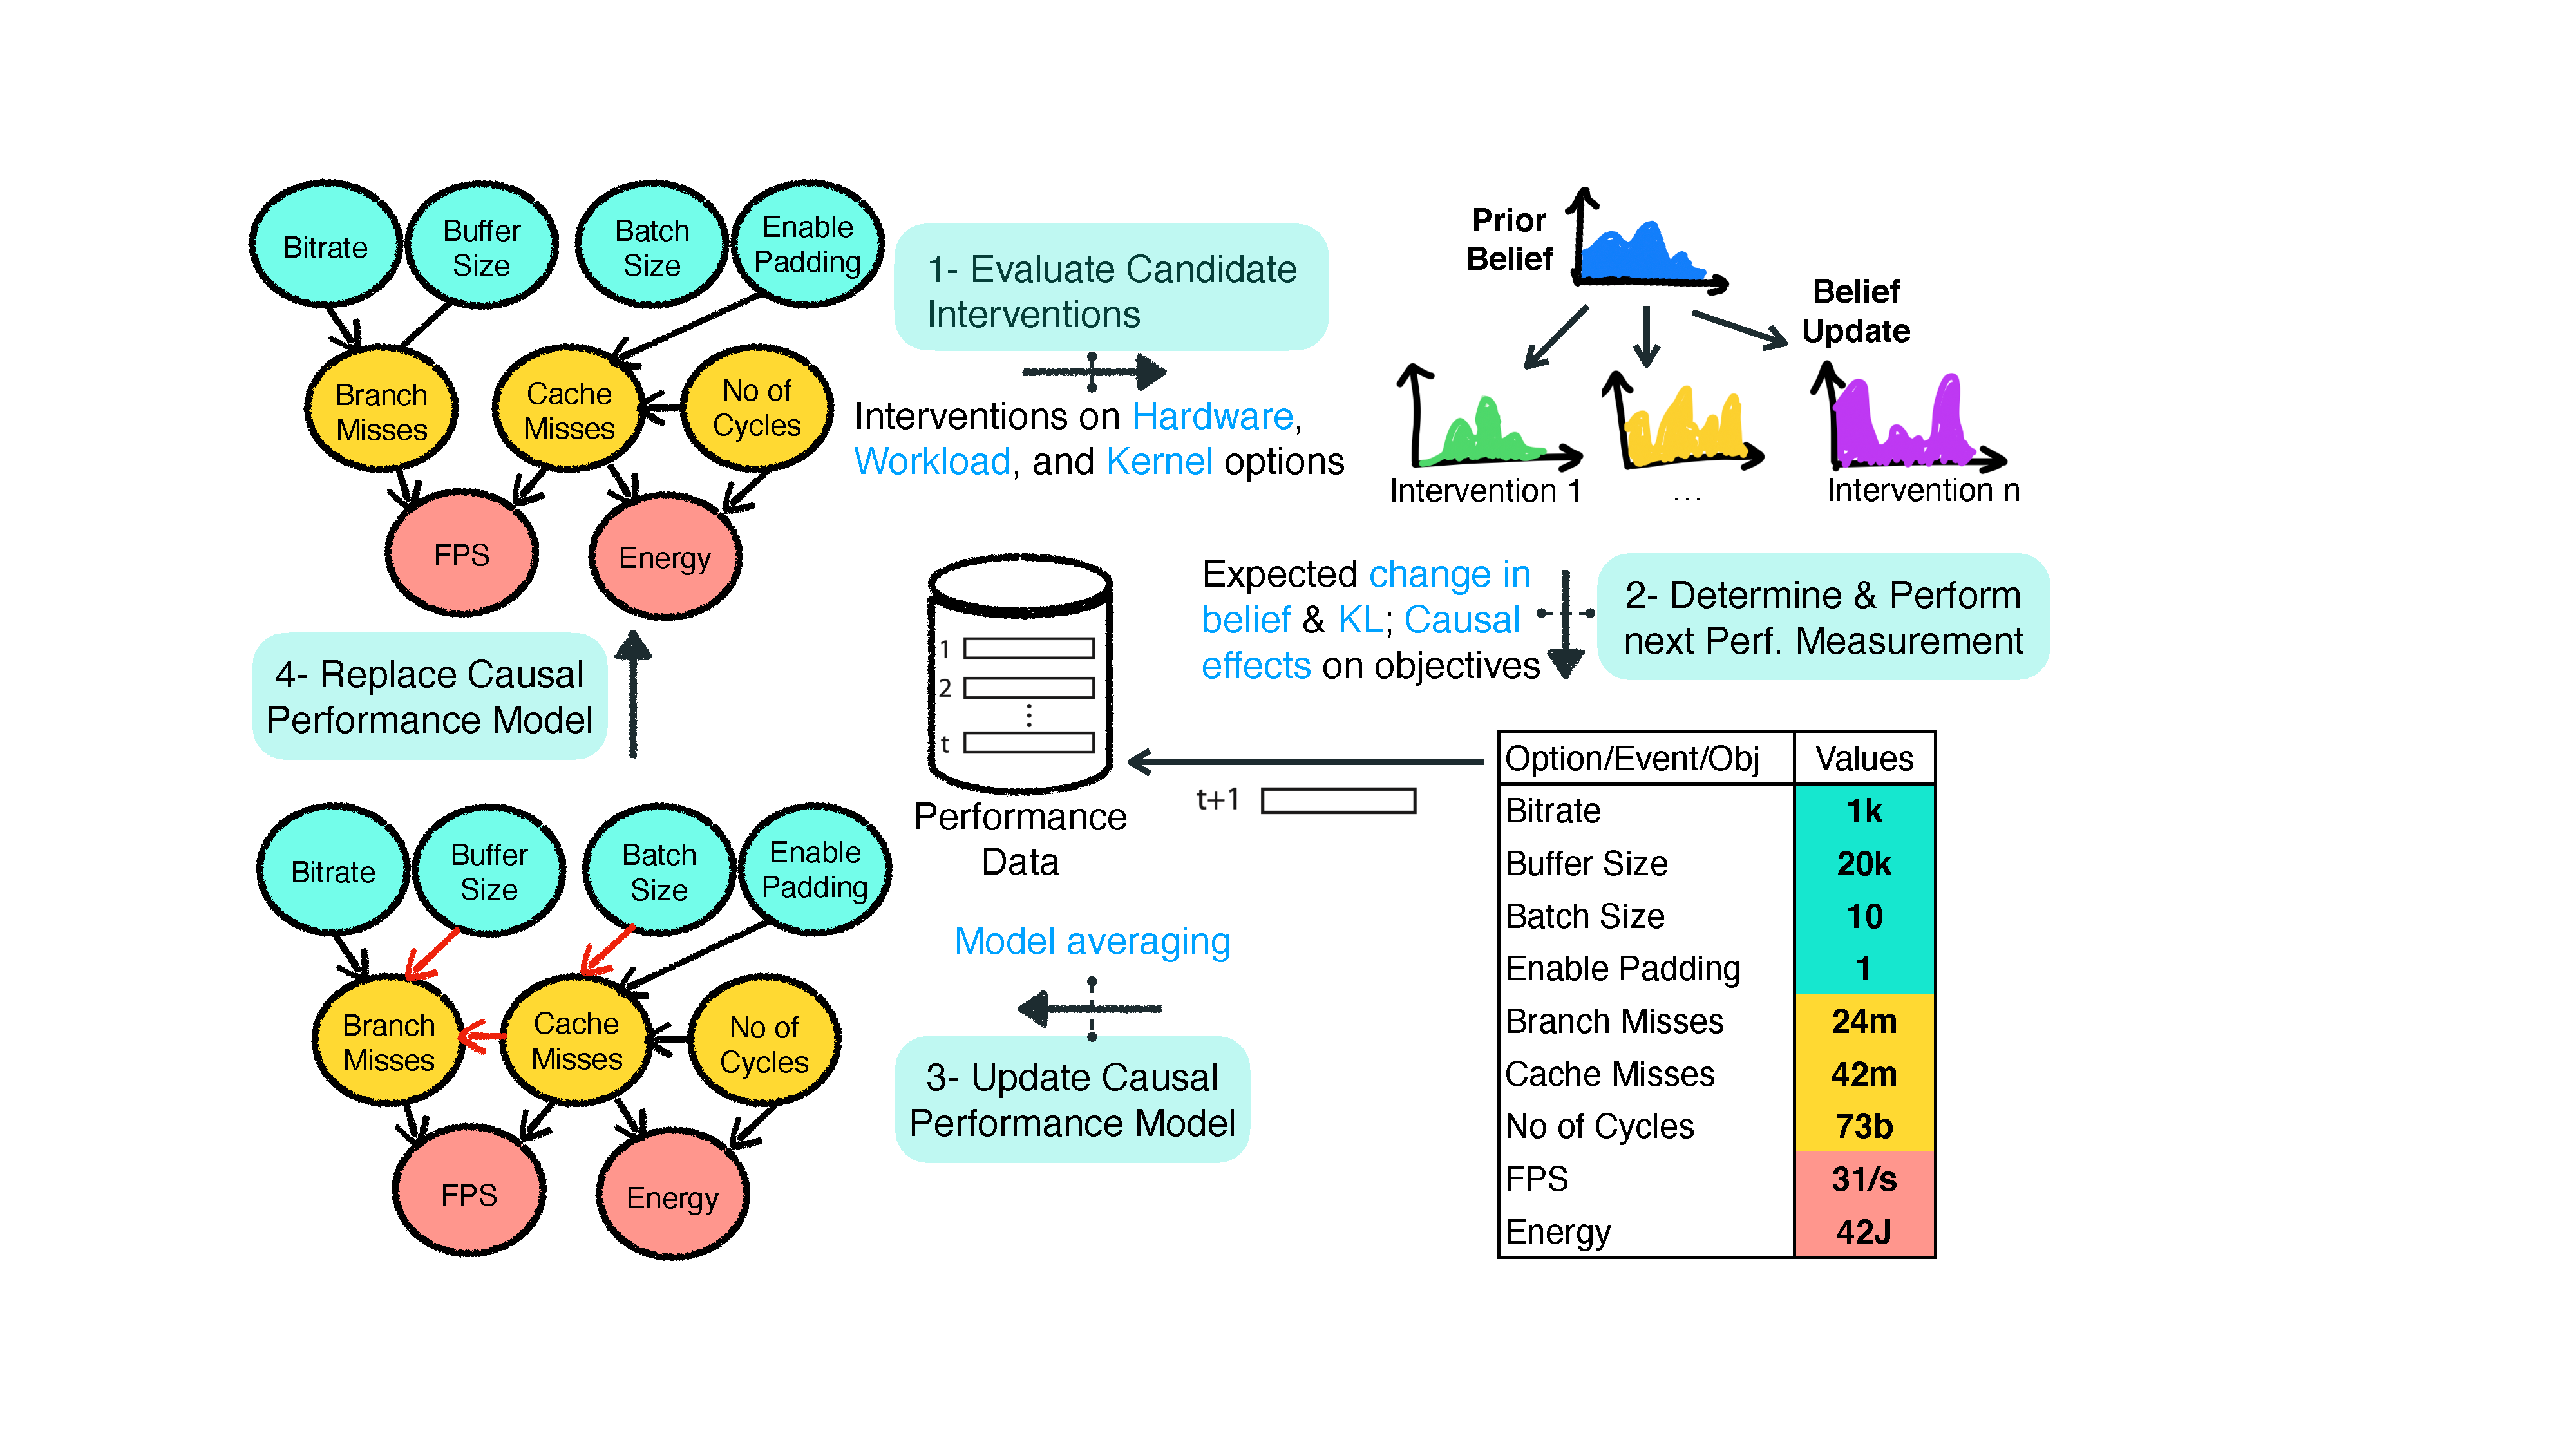
\includegraphics[width=\linewidth]{./img/Causal-Model-Update.pdf}
  \caption{\small {}}

  \label{}
\end{figure}

\section{Fallbeispiele}

In dieser Ausarbeitung werden die Ergebnisse der Evaluation von \textsc{Unicorn} anhand der Fallbeispiele aus dem Originalpaper repliziert.

\textsc{Unicorn} kann im Online- oder Offline-Modus betrieben werden. Im Online-Modus werden die Performance-Metriken direkt auf der zugrundeliegenden Hardware ausgeführt. Der Offline-Modus erlaubt die Reproduktion auf beliebiger Hardware. Da uns die im Paper genutzte Hardware nicht zur Verfügung steht, werden lediglich die Ergebnisse der Offline-Evaluation repliziert.

Die Autoren stellen den Quellcode als Python-Bibliothek auf GitHub zur Verfügung.\footnote{\href{https://github.com/softsys4ai/unicorn}{https://github.com/softsys4ai/unicorn}} Eine Dokumentation sowie eine ausführliche Anweisungen zur Replikation der Ergebnisse sind im Repository angehängt. Entsprechend den Anweisungen wurde Docker in Version \texttt{20.10.16} auf den Testsystemen installiert.

Bis auf ein fehlendes Paket, das zur Ausführung auf unseren Systemen notwendig war, konnten die Tests ohne Probleme ausgeführt werden. \textsc{Unicorn} erzeugt nach dem Testläufen mit \texttt{matplotlib} Graphen. In manchen Fällen konnten die Graphen nicht gespeichert werden, was jedoch nicht auf die eigentlichen Tests und deren Ergebnisse zurückzuführen ist.

Die Replikation findet auf zwei Testsystemen statt:\footnote{Die Testsysteme werden im Folgenden kurz als \texttt{Win} und \texttt{Mac} bezeichnet.}
\begin{itemize}
  \itemsep0em
  \item \texttt{Windows 10 21H2} mit \texttt{Intel Core i7-8700K CPU @ 12x3.50 GHz} und \texttt{32GB DDR4 RAM @ 3280Mhz}
  \item \texttt{MacOS Monterey 12.4} mit \texttt{Apple M1 CPU @ 4x3.20 GHz} und \texttt{16 GB LPDDR-DDR4X RAM @ 4266 Mhz}
\end{itemize}
Den Docker-Containern werden je 4 CPU-Kerne und 8 GB Arbeitsspeicher zur Verfügung gestellt.

Das System der Autoren im Offline-Mode verwendet als Prozessor \texttt{Intel Core i7-8700 CPU @ 12x3.20 GHz} und besitzt \texttt{31.2 GB} an Arbeitsspeicher, die zugrundeliegende Hardware ist zu unserem ersten System sehr ähnlich. Als Betriebssystem verwenden die Autoren jedoch \texttt{Ubuntu 18.04}.

Wir werden im Folgenden die Resultate der drei Kernbehauptungen des Originalpapers reproduzieren:

\begin{itemize}
  \itemsep0em
  \item \textsc{Unicorn} kann für das Aufsprüren der Ursachen von nicht-funktionalen Fehlern (Latenz, Energieverbrauch) genutzt werden.
  \item \textsc{Unicorn} kann als Werzeug bei der Durchführung von Performanceoptimierungen unterstützen.
  \item \textsc{Unicorn} ist effizient, auch wenn sich das Einsatzenvironment ändert.
\end{itemize}

\section{Replikation der Ergebnisse}

Für die Reproduktion der Ergebnisse werden die Anweisungen der Dokumentation in \texttt{artifact/REPRODUCE.md} genutzt. Leider konnten bei einigen der Experimente die von \textsc{Unicorn} ausgegeben Graphen nicht gespeichert werden, so dass der zeitliche Verlauf beispielsweise bei der Optimierung nicht ersichtlich ist.

\subsection{Erkennung der Ursachen für hohen Energieverbrauch}\label{sec:1}

In diesem Experiment soll die Ursache für den hohen Energieverbrauch ermittelt und eine Lösung hierfür gefunden werden.

\begin{figure}[tp!]
  \centering
  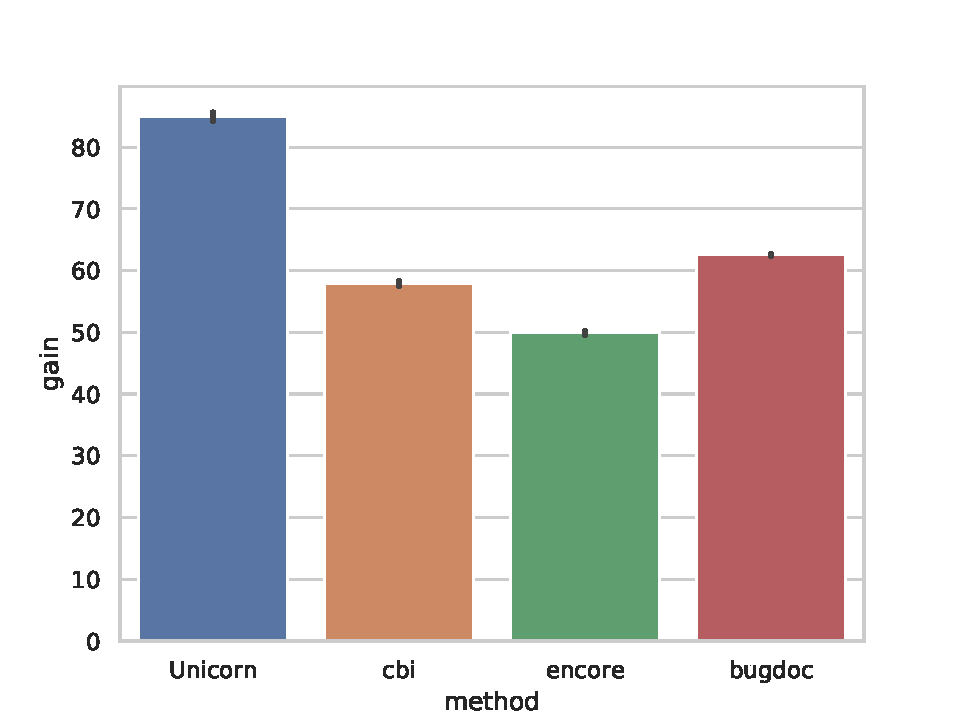
\includegraphics[width=\linewidth]{./img/win_debug_gain.pdf}
  \caption{Verbesserung des Energieverbrauchs gegenüber Standardkonfiguration bei Einsatz von \textsc{Unicorn}, CBI, \textsc{EnCore} und \textsc{BugDoc}. Die Ergebnisse sind für \texttt{Win} und \texttt{Mac} identisch.}

  \label{fig:1}
\end{figure}

\begin{figure}[tp!]
  \centering
  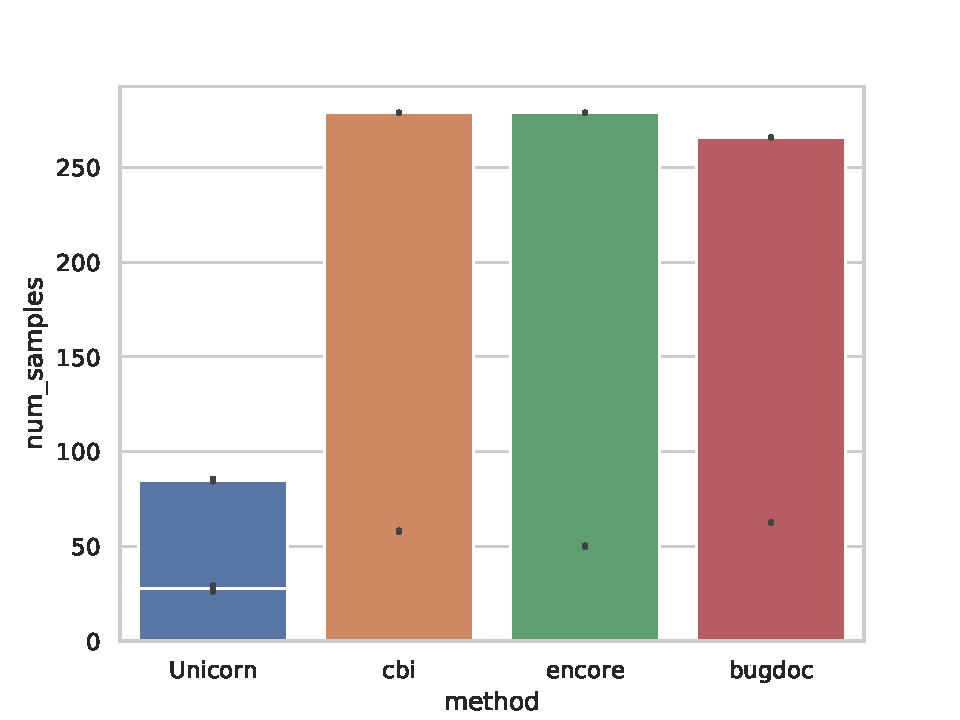
\includegraphics[width=\linewidth]{./img/win_debug_num_samples.pdf}
  \caption{Notwendige Anzahl an Samples}

  \label{fig:3}
\end{figure}

\begin{figure}[tp!]
  \centering
  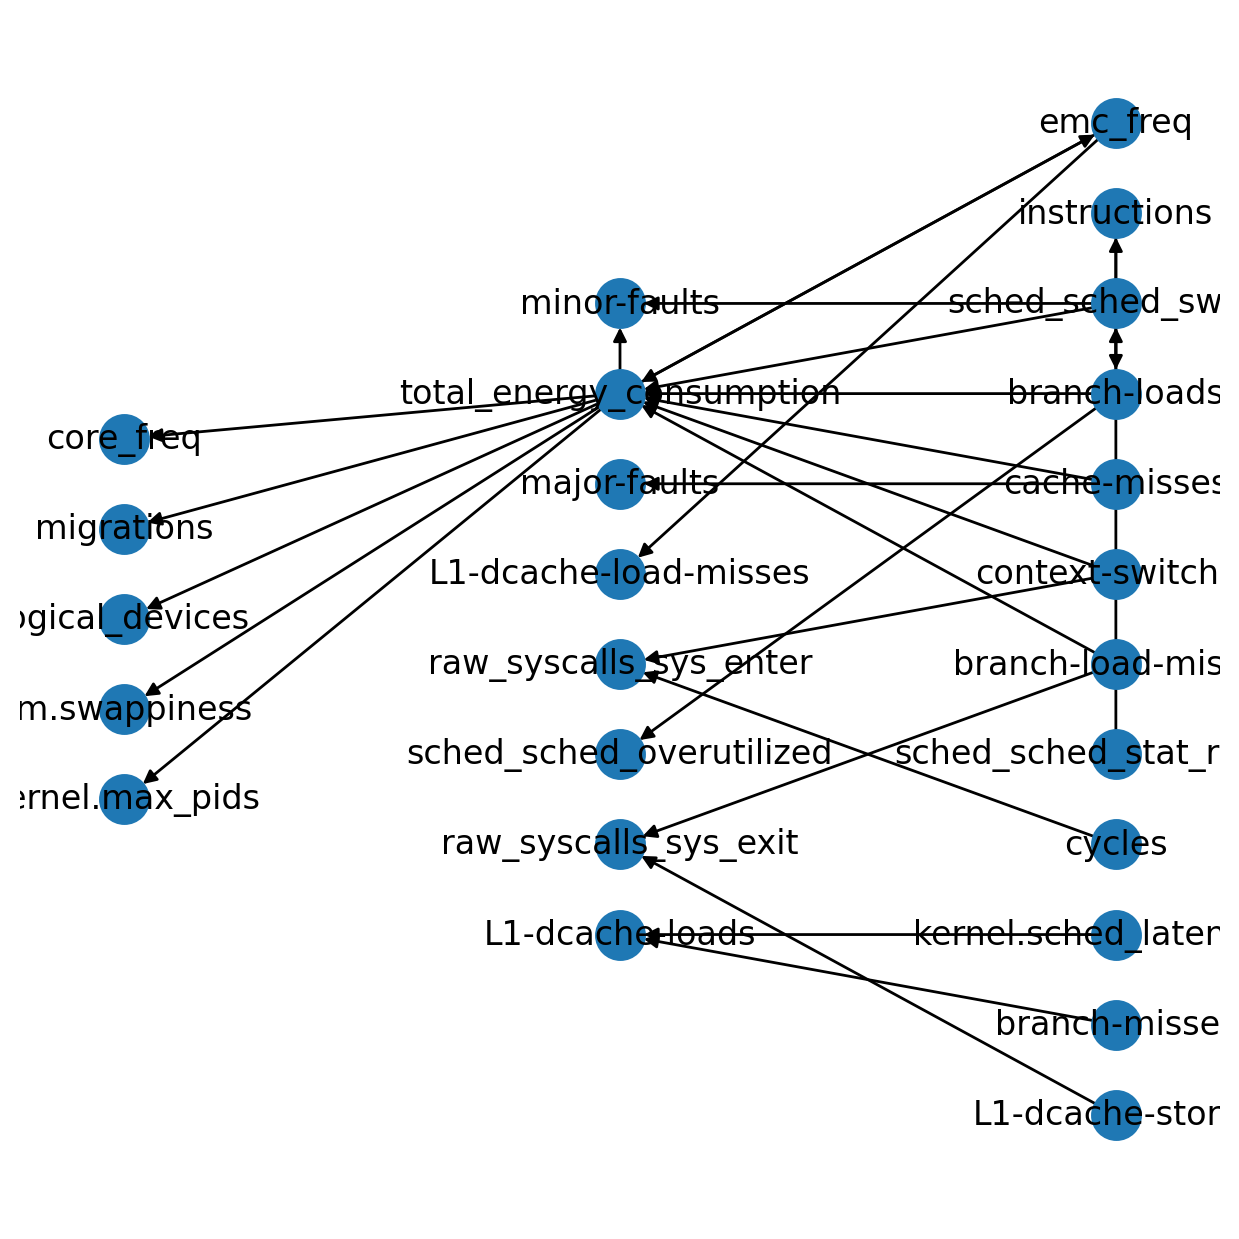
\includegraphics[width=\linewidth]{./img/causal_graph.png}
  \caption{Von \textsc{Unicorn} gelernter kausaler Graph des Experiments aus Abschnitt \ref{sec:1}.}

  \label{fig:2}
\end{figure}

Wie in Abbildung \ref{fig:1} zu sehen ist, entspricht der \textit{Gain}, d.\,h. der Zuwachs an Performance und somit die Verringerung des Energieverbrauchs, bei unseren Experimenten den Ergebnissen der Autoren. Der in Abbildung \ref{fig:2} gezeigte kausale Graph gibt Aufschluss darüber, welche Konfigurationsparameter Einfluss auf den Energieverbrauch haben. Die genauen Werte sind im von \textsc{Unicorn} ausgegeben Log zu sehen:

\begin{Verbatim}[fontsize=\small,samepage=true]
+++++++++++++++++Bug+++++++++++++++++++++
memory_growth                         0.5
logical_devices                       1.0
core_freq                       1651200.0
gpu_freq                        1651200.0
emc_freq                      800000000.0
num_cores                             2.0
scheduler.policy                      1.0
vm.swappiness                       100.0
vm.vfs_cache_pressure               500.0
vm.dirty_background_ratio            80.0
vm.drop_caches                        3.0
vm.nr_hugepages                       1.0
vm.overcommit_ratio                  50.0
vm.overcommit_memory                  1.0
vm.overcommit_hugepages               2.0
kernel.sched_child_runs_first         0.0
kernel.sched_rt_runtime_us       500000.0
vm.dirty_bytes                       30.0
vm.dirty_background_bytes            60.0
vm.dirty_ratio                        5.0
swap_memory                           1.0
kernel.max_pids                   32768.0
kernel.sched_latency_ns        24000000.0
kernel.sched_nr_migrate             256.0
kernel.cpu_time_max_percent          50.0
kernel.sched_time_avg_ms           1000.0
Name: 28, dtype: float64
Bug Objective Value 141401
\end{Verbatim}

\begin{Verbatim}[fontsize=\small,samepage=true]
+++++++++++Recommended Fix++++++++++++++
memory_growth                 5.0000e-01
logical_devices               1.0000e+00
core_freq                     1.5744e+06
gpu_freq                      1.6512e+06
emc_freq                      2.1330e+09
num_cores                     2.0000e+00
scheduler.policy              1.0000e+00
vm.swappiness                 1.0000e+02
vm.vfs_cache_pressure         5.0000e+02
vm.dirty_background_ratio     8.0000e+01
vm.drop_caches                3.0000e+00
vm.nr_hugepages               1.0000e+00
vm.overcommit_ratio           5.0000e+01
vm.overcommit_memory          1.0000e+00
vm.overcommit_hugepages       2.0000e+00
kernel.sched_child_runs_first 0.0000e+00
kernel.sched_rt_runtime_us    5.0000e+05
vm.dirty_bytes                3.0000e+01
vm.dirty_background_bytes     6.0000e+01
vm.dirty_ratio                5.0000e+00
swap_memory                   1.0000e+00
kernel.max_pids               6.5536e+04
kernel.sched_latency_ns       2.4000e+07
kernel.sched_nr_migrate       2.5600e+02
kernel.cpu_time_max_percent   5.0000e+01
kernel.sched_time_avg_ms      1.0000e+03
Name: 0, dtype: float64
Unicorn Fix Value 26678
Number of Samples Required 26
\end{Verbatim}

Wie zu erwarten schlägt \textsc{Unicorn} Änderungen bei den Frequenzen (\texttt{core\_freq}, \texttt{gpu\_freq} und \texttt{emc\_freq}) vor. Die Ergebnisse der Autoren konnten in diesem Fall sehr gut repliziert werden.

\subsection{Optimierung der Inferenzzeit}

In diesem Experiment wird die minimale Latenz, d.\,h. die Inferenzzeit, optimiert.

Das lokale Optimum von 12 Sekunden Inferenzzeit erreicht \textsc{Unicorn} bereits nach 69 Iterationen. Auf \texttt{Win} benötigt es dafür ca. 280 Minuten, auf \texttt{Mac} benötigt es 70 Minuten, die nötige Laufzeit von Unicorn auf \texttt{Win} war also sehr viel länger war als auf \texttt{Mac} und damit deutlich länger als in der Dokumentation angegeben (ca. 90 Minuten). Grundsätzlich ist hierbei nicht davon auszugehen, dass die zugrundeliegende Hardware dafür verantwortlich ist, da die Autoren bei ihren Experimenten die gleiche CPU verwendet haben. Möglicherweise ist eine Systemkonfiguration außerhalb des Containers, in dem die Berechnungen stattfanden, dafür verantwortlich (Docker von \texttt{Win} basiert auf WSL2 was beim Testsystem der Autoren, das auf Ubuntu basiert, nicht der Fall ist).

Auch hier stimmen die Resultate mit denen im Paper überein. \textsc{Unicorn} erreicht das lokale Optimum bereits nach 69 Iterationen und damit schneller als SMAC. Andererseits ist das von \textsc{Unicorn} gefundene Optimum um 8 Sekunden besser als das von SMAC.






\subsection{Änderung der Hardware}

In diesem Experiment wird die Übertragbarkeit des von \textsc{Unicorn} gelernten Modells untersucht.



\newpage
\newpage



The templates include the \LaTeX{} source of this document (\texttt{acl.tex}),
the \LaTeX{} style file used to format it (\texttt{acl.sty}),
an ACL bibliography style (\texttt{acl\_natbib.bst}),
an example bibliography (\texttt{custom.bib}),
and the bibliography for the ACL Anthology (\texttt{anthology.bib}).

\section{Engines}

To produce a PDF file, pdf\LaTeX{} is strongly recommended (over original \LaTeX{} plus dvips+ps2pdf or dvipdf). Xe\LaTeX{} also produces PDF files, and is especially suitable for text in non-Latin scripts.

\section{Preamble}

The first line of the file must be
\begin{quote}
\begin{verbatim}
\documentclass[11pt]{article}
\end{verbatim}
\end{quote}

To load the style file in the review version:
\begin{quote}
\begin{verbatim}
\usepackage[review]{acl}
\end{verbatim}
\end{quote}
For the final version, omit the \verb|review| option:
\begin{quote}
\begin{verbatim}
\usepackage{acl}
\end{verbatim}
\end{quote}

To use Times Roman, put the following in the preamble:
\begin{quote}
\begin{verbatim}
\usepackage{times}
\end{verbatim}
\end{quote}
(Alternatives like txfonts or newtx are also acceptable.)

Please see the \LaTeX{} source of this document for comments on other packages that may be useful.

Set the title and author using \verb|\title| and \verb|\author|. Within the author list, format multiple authors using \verb|\and| and \verb|\And| and \verb|\AND|; please see the \LaTeX{} source for examples.

By default, the box containing the title and author names is set to the minimum of 5 cm. If you need more space, include the following in the preamble:
\begin{quote}
\begin{verbatim}
\setlength\titlebox{<dim>}
\end{verbatim}
\end{quote}
where \verb|<dim>| is replaced with a length. Do not set this length smaller than 5 cm.

\section{Document Body}

\subsection{Footnotes}

Footnotes are inserted with the \verb|\footnote| command.\footnote{This is a footnote.}

\subsection{Tables and figures}

See Table~\ref{tab:accents} for an example of a table and its caption.
\textbf{Do not override the default caption sizes.}

\begin{table}
\centering
\begin{tabular}{lc}
\hline
\textbf{Command} & \textbf{Output}\\
\hline
\verb|{\"a}| & {\"a} \\
\verb|{\^e}| & {\^e} \\
\verb|{\`i}| & {\`i} \\
\verb|{\.I}| & {\.I} \\
\verb|{\o}| & {\o} \\
\verb|{\'u}| & {\'u}  \\
\verb|{\aa}| & {\aa}  \\\hline
\end{tabular}
\begin{tabular}{lc}
\hline
\textbf{Command} & \textbf{Output}\\
\hline
\verb|{\c c}| & {\c c} \\
\verb|{\u g}| & {\u g} \\
\verb|{\l}| & {\l} \\
\verb|{\~n}| & {\~n} \\
\verb|{\H o}| & {\H o} \\
\verb|{\v r}| & {\v r} \\
\verb|{\ss}| & {\ss} \\
\hline
\end{tabular}
\caption{Example commands for accented characters, to be used in, \emph{e.g.}, Bib\TeX{} entries.}
\label{tab:accents}
\end{table}

\subsection{Hyperlinks}

Users of older versions of \LaTeX{} may encounter the following error during compilation:
\begin{quote}
\tt\verb|\pdfendlink| ended up in different nesting level than \verb|\pdfstartlink|.
\end{quote}
This happens when pdf\LaTeX{} is used and a citation splits across a page boundary. The best way to fix this is to upgrade \LaTeX{} to 2018-12-01 or later.

\subsection{Citations}

\begin{table*}
\centering
\begin{tabular}{lll}
\hline
\textbf{Output} & \textbf{natbib command} & \textbf{Old ACL-style command}\\
\hline
\citep{Gusfield:97} & \verb|\citep| & \verb|\cite| \\
\citealp{Gusfield:97} & \verb|\citealp| & no equivalent \\
\citet{Gusfield:97} & \verb|\citet| & \verb|\newcite| \\
\citeyearpar{Gusfield:97} & \verb|\citeyearpar| & \verb|\shortcite| \\
\hline
\end{tabular}
\caption{\label{citation-guide}
Citation commands supported by the style file.
The style is based on the natbib package and supports all natbib citation commands.
It also supports commands defined in previous ACL style files for compatibility.
}
\end{table*}

Table~\ref{citation-guide} shows the syntax supported by the style files.
We encourage you to use the natbib styles.
You can use the command \verb|\citet| (cite in text) to get ``author (year)'' citations, like this citation to a paper by \citet{Gusfield:97}.
You can use the command \verb|\citep| (cite in parentheses) to get ``(author, year)'' citations \citep{Gusfield:97}.
You can use the command \verb|\citealp| (alternative cite without parentheses) to get ``author, year'' citations, which is useful for using citations within parentheses (e.g. \citealp{Gusfield:97}).

\subsection{References}

\nocite{Ando2005,borschinger-johnson-2011-particle,andrew2007scalable,rasooli-tetrault-2015,goodman-etal-2016-noise,harper-2014-learning}

The \LaTeX{} and Bib\TeX{} style files provided roughly follow the American Psychological Association format.
If your own bib file is named \texttt{custom.bib}, then placing the following before any appendices in your \LaTeX{} file will generate the references section for you:
\begin{quote}
\begin{verbatim}
\bibliographystyle{acl_natbib}
\bibliography{custom}
\end{verbatim}
\end{quote}

You can obtain the complete ACL Anthology as a Bib\TeX{} file from \url{https://aclweb.org/anthology/anthology.bib.gz}.
To include both the Anthology and your own .bib file, use the following instead of the above.
\begin{quote}
\begin{verbatim}
\bibliographystyle{acl_natbib}
\bibliography{anthology,custom}
\end{verbatim}
\end{quote}

Please see Section~\ref{sec:bibtex} for information on preparing Bib\TeX{} files.

\subsection{Appendices}

Use \verb|\appendix| before any appendix section to switch the section numbering over to letters. See Appendix~\ref{sec:appendix} for an example.

\section{Bib\TeX{} Files}
\label{sec:bibtex}

Unicode cannot be used in Bib\TeX{} entries, and some ways of typing special characters can disrupt Bib\TeX's alphabetization. The recommended way of typing special characters is shown in Table~\ref{tab:accents}.

Please ensure that Bib\TeX{} records contain DOIs or URLs when possible, and for all the ACL materials that you reference.
Use the \verb|doi| field for DOIs and the \verb|url| field for URLs.
If a Bib\TeX{} entry has a URL or DOI field, the paper title in the references section will appear as a hyperlink to the paper, using the hyperref \LaTeX{} package.

\section*{Acknowledgements}

This document has been adapted
by Steven Bethard, Ryan Cotterell and Rui Yan
from the instructions for earlier ACL and NAACL proceedings, including those for
ACL 2019 by Douwe Kiela and Ivan Vuli\'{c},
NAACL 2019 by Stephanie Lukin and Alla Roskovskaya,
ACL 2018 by Shay Cohen, Kevin Gimpel, and Wei Lu,
NAACL 2018 by Margaret Mitchell and Stephanie Lukin,
Bib\TeX{} suggestions for (NA)ACL 2017/2018 from Jason Eisner,
ACL 2017 by Dan Gildea and Min-Yen Kan,
NAACL 2017 by Margaret Mitchell,
ACL 2012 by Maggie Li and Michael White,
ACL 2010 by Jing-Shin Chang and Philipp Koehn,
ACL 2008 by Johanna D. Moore, Simone Teufel, James Allan, and Sadaoki Furui,
ACL 2005 by Hwee Tou Ng and Kemal Oflazer,
ACL 2002 by Eugene Charniak and Dekang Lin,
and earlier ACL and EACL formats written by several people, including
John Chen, Henry S. Thompson and Donald Walker.
Additional elements were taken from the formatting instructions of the \emph{International Joint Conference on Artificial Intelligence} and the \emph{Conference on Computer Vision and Pattern Recognition}.

% Entries for the entire Anthology, followed by custom entries
\bibliography{anthology,custom}
\bibliographystyle{acl_natbib}

\appendix

\section{Example Appendix}
\label{sec:appendix}

This is an appendix.

\end{document}
